\documentclass[]{article}
\usepackage[utf8]{inputenc}
\usepackage[T1]{fontenc}
\usepackage[usenames,dvipsnames,pdftex]{xcolor}
\usepackage[upright]{fourier}
\usepackage[english]{babel}
\usepackage{hyperref}
\usepackage{calc}
\usepackage{amsmath}
\usepackage{amssymb}
\usepackage{mathrsfs}
\usepackage{amsthm}
\usepackage{fullpage}
\usepackage{tkz-graph}

\title{TP d'Algo/Complexité/Calculabilité}
\author{
  CIMBE Pierre-Alexandre \\
  LAGNIEZ Jean-Marc \\
  LESNYAK Viktor \\
  RAFIK Ahmed}
\date\today

\begin{document}

\maketitle

\section{Partie théorique}
\subsection{Partie algorithmique}

\subsubsection{Exercice 1}

\begin{enumerate}

\item Le nombre de s-t chemins d'arc disjoint est de 3.\\
On trouve ce résultat en appliquant l'algorithme de Ford-Fulkerson.\\
\begin{center}
s -> 4 -> 5 -> t      F = 1\\
s -> 3 -> 4 -> t      F = 1\\
s -> 2 -> 3 -> t      F = 1\\
\end{center}
Tous les arcs du graphe sont saturés donc on ne peut plus trouver de chemin améliorant et Fmax = 3.\\


\item Soit Si l'ensemble des sommets de la coupe i, $\overline Si$ l'ensemble des sommets du complémentaire de la coupe i, \\
Avi l'ensemble des arcs avants de la coupe i, et Ari l'ensemble des arcs arrière de cette coupe.\\
\begin{center}
S1 = \{1\} ; $\overline S1$ = \{2, 3, 4, 5, 6\}\\ 
Av1 = \{1->4 ; 1->3 ; 1->2\} ; Ar1 = \{\}\\
S2 = \{1, 2\} ; $\overline S2$ = \{3, 4, 5, 6\}\\
Av2 = \{1->4 ; 1->3 ; 2->3\} ; Ar2 = \{\}\\ 
S3 = \{1, 4\} ; $\overline S3$ = \{2, 3, 5, 6\}\\
Av3 = \{1->3 ; 1->2 ; 4->5 ; 4->6\} ; Ar3 = \{3->4\}\\
S4 = \{1, 2, 3\} ; $\overline S4$ = \{4, 5, 6\}\\ 
Av4 = \{1->4 ; 3->4 ; 3->6\} ; Ar4 = \{\}\\
S5 = \{1, 2, 4\} ; $\overline S5$ = \{3, 5, 6\}\\
Av5 = \{1->3 ; 2->3 ; 4->5 ; 4->6\} ; Ar5 = \{3->4\}\\
S6 = \{1, 4, 5\} ; $\overline S6$ = \{2, 3, 6\}\\
Av6 = \{1->2 ; 1->3 ; 4->6 ; 5->6\} ; Ar6 = \{3->4\}\\ 
S7 = \{1, 2, 3, 4\} ; $\overline S7$ = \{5, 6\}\\ 
Av7 = \{4->5 ; 4->6 ; 3->6\} ; Ar6 = \{\}\\ 
S8 = \{1, 2, 3, 4, 5\} ; $\overline S8$ = \{6\}\\
Av6 = \{3->6 ; 4->6 ; 5->6\} ; Ar6 = \{\}\\
\end{center}


\item Nombre minimum d'arc sortant dans une s-t coupe = 3\\
  Nombre maximum de chemin d'arc disjoint = 3\\


\subsubsection{Exercice 2}

\textbf{Soit un graphe G=(V,E);\\avec $\forall i,j \in V$,\\
et f(i,j)-est la fonction representant le flot de l'arc ou $\forall (i,j)\in E$;\\}

\begin{enumerate}


\item Vrai, car si on enleve un arc (i,j), avec la f(i,j)=0,\\ alors on n'influence pas la valeur du flot maximal.\\
Ce qui correspondt a la definition de plus petit \\arc vital.

\item Vrai, car dans un flot maximum un arc (i,j) avec le f(i,j)\\ minimum est le plus petit arc vital d'apres la \\
definition de plus petit arc vital.
\item Faux, voila un contre exemple.


\usetikzlibrary{arrows}
\thispagestyle{empty}
\begin{center}
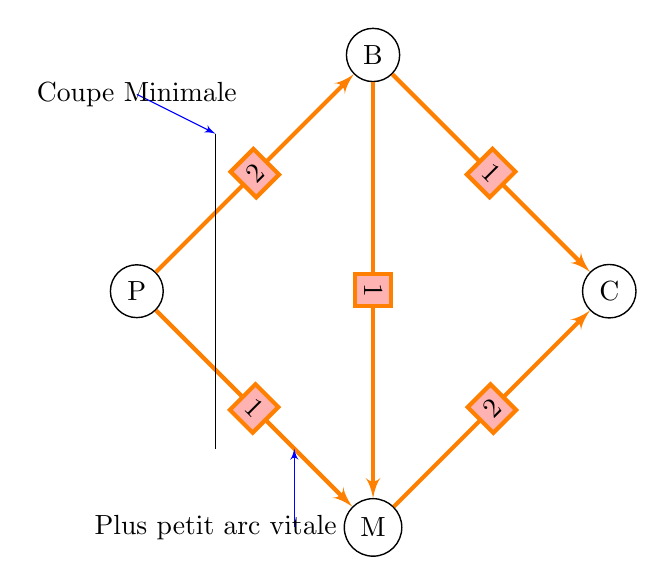
\begin{tikzpicture}[>=latex']
 \SetUpEdge[lw         = 1.5pt,
            color      = orange,
            labelcolor = red!30,
            labelstyle = {draw,sloped}]
  \tikzset{node distance = 5cm}
  \GraphInit[vstyle=Normal]
  \Vertex[x=-3, y=0]{P}
  \Vertex[x=0, y=3]{B}
  \Vertex[x=3, y=0]{C}
  \Vertex[x=0, y=-3]{M}
  \tikzset{EdgeStyle/.style={->}}
  \Edge[label=$2$](P)(B)
  \Edge[label=$1$](P)(M)
  \Edge[label=$1$](B)(C)
  \Edge[label=$2$](M)(C)
  \Edge[label=$1$](B)(M)
  \draw (-2,2) -- (-2,-2);
  \draw[blue,->](-1,-3)--(-1,-2);
  \draw[blue,->](-3,2.5)--(-2,2);

  \node at (-3,2.5){Coupe Minimale};
  \node at (-2,-3){Plus petit arc vitale};
\end{tikzpicture}
\end{center}
 
\end{enumerate} 
\subsubsection{Exercice 3}

\begin{enumerate}


\item Donc pour la partie recherche : trouver un sous-graphe d'un graphe $K2n+1$ qui est isomorphe a une double etoile on peut donner un\\
example avec le graphe de petersen(voila le lien : $http://fr.wikipedia.org/wiki/Graphe\_de\_Petersen$);

\item Pour la partie de demonstration : en considerant le +1 (de la formule $K2n+1$) comme le sommet racine, on peut \\
dire que nous avons un graphe bipartie, et donc on peut trouver une equivalence avec le probleme d'affectation(le \\
probleme de couplage maximum de poids minimum).

\end{enumerate}


\subsection{Partie complexité}

\subsubsection{Exercie 5}

\begin{enumerate}
\item 
  \begin{enumerate}
  \item
    SAT : Un  problème SAT est un problème de décision visant à montrer l'existence d'une interprétation satisfaisant un ensemble de variable propositionnelle (Formule logique CNF)\\
    3-SAT : Cas particulier du problème SAT dans lequel les clauses sont toutes de taille 3.\\

  \item
    On dit qu'il existe une réduction d'un problème P à un problème P' s'il existe une fonction f telle que x $\in$ D(P) <=> f(x) $\in$ D(P')\\

  \item
    3-SAT est un cas particulier de SAT, or SAT $\in$ NP.\\
    Donc 3-SAT $\in$ NP

    SAT $\in$ NP-Complet

    Nous allons chercher à réduire un problème SAT à un problème 3-SAT : 

    Soit P une instance du problème SAT.
    
    $\twoheadrightarrow$Soit U={$l_1vl_2vl_3......vl_k$} une clause de taille k > 3

    On la divise en 2 clause :
    $\succ$ une clause de taille $\lfloor$k/2$\rfloor$+1 en complétant par une variable x$\notin$U 
    $\succ$ une clause de taille $\lceil$k/2$\rceil$+1 en complétant par $\overline x$ le complémentaire de x.

    On applique ce principe récursivement jusqu'à obtenir des clauses de taille 3

    $\twoheadrightarrow$Soit U={$l_1vl_2$} une clause de taille 2
    
    On clone la clause U pour avoir 2 clauses $U_1$ et $U_2$ auxquelles on ajoute respectivement une variable x et son complémentaire $\overline x$
    on obtient :  $U_1$={$l_1vl_2$vx}
    $U_2$={$l_1vl_2$v$\overline x$}

    $\twoheadrightarrow$Soit U={$l_1$} une clause de taille 1
    On force $l_1$ à vrai et on retire les clauses unitaire.

    On obtient ainsi un problème P' de type 3-SAT.    

    Donc 3-SAT est NP-Complet.\\

    \item
      Clause de taille 4 :\\
      Soit $l_1$, $l_2$, $l_3$, $l_4$ une clause de taille 4

      \begin{center}
      $l_1$, $l_2$, $l_3$, $l_4$ \left\lbrace 
      \begin{array}{lcl} 
        l_1 v l_2 v u\\
        l_3 v l_4 v \overline u
      \end{array}\right.
      \end{center}

      Chaque clause contenant 4 littéraux est ainsi divisée en 2 clauses de 3 littéraux
      \begin{center}
        n_4 -> 2n_4
      \end{center}
      On ajoute ainsi une variable pour chaque clause
      \begin{center}
        4n_4 -> 5n_4
      \end{center}
      \newline

      Clause de taille 5 :\\      
      Soit $l_1$, $l_2$, $l_3$, $l_4$, $l_5$ une clause de taille 5

      \begin{center}
      $l_1$, $l_2$, $l_3$, $l_4$, $l_5$\left\lbrace 
      \begin{array}{lcl} 
        l_1 v l_2 v u\\
        l_3 v l_4 v l_5 v \overline u
      \end{array}\right.
      \end{center}

      \begin{center}
      $l_3$ v $l_4$ v $l_5$ v \overline u\left\lbrace 
      \begin{array}{lcl} 
        l_3 v l_4 v y\\
        l_5 v \overline u v \overline y
      \end{array}\right.
      \end{center}

      Chaque clause contenant 5 littéraux est ainsi divisée en 3 clauses de 3 littéraux
      \begin{center}
        n_5 -> 3n_5
      \end{center}
      On ajoute ainsi 2 variables pour chaque clause
      \begin{center}
        5n_5 -> 7n_5
      \end{center}
      \newline

      Clause de taille 2 :\\
      Soit $l_1$, $l_2$ une clause de taille 2

      \begin{center}
      $l_1$, $l_2$\left\lbrace 
      \begin{array}{lcl} 
        l_1 v l_2 v u\\
        l_1 v l_2 v \overline u
      \end{array}\right.
      \end{center}

      Chaque clause contenant 2 littéraux est transformée en 2 clauses de 3 littéraux
      \begin{center}
        n_2 -> 2n_2
      \end{center}
      On ajoute ainsi 1 variables pour chaque clause
      \begin{center}
        2n_2 -> 3n_2
      \end{center}
      \newline


      Clause de taille 1 :\\
      Soit $l_1$ une clause de taille 1

      \begin{center}
      $l_1$\left\lbrace 
      \begin{array}{lcl} 
        l_1 v u v \overline u
      \end{array}\right.
      \end{center}

      Chaque clause contenant 1 littéraux est transformée en une clause de 3 littéraux
      \begin{center}
        n_1 -> n_1
      \end{center}
      On ajoute ainsi 1 variables pour chaque clause
      \begin{center}
        n_1 -> 3n_1
      \end{center}
      \newline

      On peut donc conclure :
      \begin{center}
        Nombre de clauses = n_1 + 3n_2 + n_3 + 2n_4 + 3n_5\\
        Nombre de variables = 3n_1 + 3n_2 + 3n_3 + 5n_4 + 7n_5\\
      \end{center}

\end{enumarate}


      


    
\end{enumerate}
\end{enumerate}



\subsection{Partie calculabilité}



\subsubsection{Exercice 7}

\noindent\fbox{\parbox{\linewidth-2\fboxrule-2\fboxsep}{ \begin {enumerate} \scriptsize  
\item \textbf{Comment enumérer les couples d'entiers?}\\
\item \textbf{Donner les fonctions de codage et de décodage f\oldstylenums{1} $\rightarrow$ x et f\oldstylenums{2} $\rightarrow$ y}\\
\item \textbf{Montrer que l'on peut coder les triplets. Géneraliser aux k-uplets.}\\
\item \textbf{Pensez-vous que l'on peut coder les éléments de l'intervalle [0,1]. Justifier.}
\end{enumerate} }}\\\\

\begin{enumerate}
\item Soit (x,y) $\in$ $\mathbb{N}$ * $\mathbb{N}$, alors faire x + y et trié par ordre lexicographique
\item La fonction de codage est : \[z = \frac{(x+y)(x+y+1)}{2} + y\]\\
Pour les fonction de décodage, posons t tel que \[t = x + y\]
On va prendre t tel que si t augmente de 1 alors \[\frac{t(t+1)}{2} > z\] sinon on a \[\frac{t(t+1)}{2} \le z\]
La fonction de décodage de y est: \[z =\frac{t(t+1)}{2} + y\] \[y = z - \frac{t(t+1)}{2}\]
La fonction de décodage de x est: \[x = t - y\] \[x = -z + t + \frac{t(t+1)}{2}\] \[x = -z + \frac{t(t+3)}{2}\]
\item Pour coder les triplets, il suffit de coder deux entier et coder le résultat et le dernier entier. 
  \[h(x,y,z)=c(x , c(y,z))\]
On peut repeter se raisonement pour les k-uplets, ainsi on a 
\[k(x\oldstylenums{1},x\oldstylenums{2}... x\oldstylenums{k}) = c(x\oldstylenums{1} , c(x\oldstylenums{2} , ... c(x\oldstylenums{k-1},x\oldstylenums{k}))\]
\item On ne peut pas coder les éléments de l'intervalle [0,1] car l'ensemble n'est pas dénombrable. On utilise la diagonal de cantor sur cette ensemble.\\
Supposons que l'on puisse numeroter $\mathbb{N}$  $\rightarrow$ [0,1] et on en définie la suite S telle que tout éléments de [0,1] soit élément de la suite S.
Et on définie un réel r tel que la partie entière est égal à 0 et que chaque décimal en position n est égal à sn(n)\footnote{la nème décimal du nème élément de S}+1 si sn(n) est différent de 9 et sn(n)-1 si sn(n) est égal à 9.\\
Par construction, r n'est pas dans S sinon on aurait un Sn tel que \[Sn(n)=r(n)=Sn(n)+1\] ou \[Sn(n)=r(n)=Sn(n)-1\] C'est absurbe, ainsi ce n'est pas dénombrable. 
   
  
\end{enumerate}




\subsubsection{Exercice 8}
\begin{enumerate}
\item Les fonctions primitives récursives sont toutes les fonctions que l'on peut construire à partir des fonctions de base pas composition et récursion primitive.\\

  Exemple\\ \\
Soit les fonctions primitives: \\
O $\in \mathbb{N}^0$, $\pi_i^k \in \mathbb{N}^k$ et SUC $\mathbb{N}^1$ 

 \[O() = 0 \] 
\[\pi_i^k(x_1,x_2...,x_k) = x_i \] 
\[SUC(x_1) = x_1 + 1 \] 

Soit la fonction qu'on utilise pour la récursion primitive:\\
g $\in \mathbb{N}^1$
\[g() = SUC(O()) \]

Soit la fonction recursive primitive:\\
f $\in \mathbb{N}^1$
\[f(0) = g()\]
\[f(SUC(n)) = \pi_1^2(f(n),n)\]
  
\item  yoloooooooo je ne sais pas 
\item \begin{enumerate}\item Soit la fonction somme défini ainsi:\\
 Sum $\in \mathbb{N}^2$ 
\[Sum(0,y) = \pi_1^1(y) = y \]
\[Sum(Suc(x),y) = \pi_2^3(x,Sum(x,y),y)\]
\item Soit la fonction Mult défini ainsi: \\
Mult $\in \mathbb{N}^2$
\[Mult(O,y) = 0() = 0\]
\[Mult(1,y) = \pi_1^1(y) = y\]
\[Mult(Suc(x),y) = \pi_2^3(x,Sum(Mult(x,y),y),y)\]
\item Soit la fonction puissance défini aisni:\\
 $X^Y$ $\in \mathbb{N}^2$
\[X^Y(x,0) = Suc(0()) = 1\]
\[X^Y(x,Suc(y)) = \pi_2^3(x,Mult(X^Y(x,y),x),y)\]
\item Soit la fonction prédecesseurs tel que: \\
Pred $\in \mathbb{N}^1$
\[Pred(0) = O() = 0\]
\[Pred(Suc(x)) = \pi_1^2(x,Pred(x))\]
\item Soit la fonction soustraction tel que:\\
X-Y $\in \mathbb{N}^2$
\[X-Y(0,y) = 0() = 0\]
\[X-Y(x,0) = \pi_1^1(x) = x\]
\[X-Y(x,y) = \pi_2^3(x,X-Y(Pred(x),Pred(y)),y))\]
\item Soit la fonction sg tel que:
sg $\in \mathbb{N}^1$
\[sg(0) = 0() = 0\]
\[sg(Suc(x)) = \pi_1^2(1,Suc(x))\]
\item Soit la fonction X > Y tel que :\\
X>Y $\in \mathbb{N}^2$
\[X>Y(0,y) = 0\]
\[X>Y(x,0) = 1\]
\[X>Y(x,y) = \pi_2^3(x,X>Y(Pred(x),Pred(y)),y)\]
Soit la fonction X $\ge$ Y tel que :\\
X$\ge$Y $\in \mathbb{N}^2$
\[X\ge Y(0,0) = 1\]
\[X\ge Y(0,y) = 0\]
\[X\ge Y(x,0) = 1\]
\[X\ge Y(x,y) = \pi_2^3(x,X>Y(Pred(x),Pred(y)),y)\]

\end{enumerate}
\item \begin{enumerate} 

\item Voici la fonction d'Ackerman pour 0 $\le$ m $\le$ 3 et 0 $\le$ n $\le$ 4 \\
\begin{center}
\begin{tabular}{| c || c | c | c | c | c |}
\hline
m/n & 0 & 1 & 2 & 3 & 4 \\
\hline
\hline
0 & 1 & 2 & 3 & 4 & 5 \\
\hline
1 & 2 & 3 & 4 & 5 & 6 \\
\hline
2 & 3 & 5 & 7 & 9 & 11 \\
\hline
3 & 5 & 13 & 28 & 58 & 118 \\
\hline
\end{tabular}
\end{center}

\item Fesons une preuve par récurrence
\[A_0(n) = Suc(n) = n + 1\]
Hypothèse: A\tiny m\normalsize (n) est primitive récursive\\
Montrons que A\tiny m+1\normalsize (n) est primitive récursive\\ 

Si n = 0, on a que A\tiny m+1\normalsize (n) = A\tiny m\normalsize (1). D'après l'hypothèse de réccurence, on a que A\tiny m\normalsize (n) est primitive récursive. Donc A\tiny m+1\normalsize (n) est primitf recursive\\

Si n > 0, on a que A\tiny m+1\normalsize (n) = A\tiny m\normalsize (A\tiny m+1\normalsize (n)).\\
Posons n' = A\tiny m+1\normalsize (n). Donc on a A\tiny m\normalsize (n'). D'après l'hypothèse de réccurence, on a que A\tiny m\normalsize (n) est primitive récursive pour tous n $\in \mathbb{N}$ . Donc A\tiny m+1\normalsize (n) est primitif recursive.\\

\item 
Fesons une preuve par récurrence 
\[A_0(n) = n+1 \] 
n+1 > n donc c'est vrai au premier rang\\
Hypothèse: A\tiny m\normalsize (n) > n \\
Montrons que A\tiny m+1\normalsize (n) > n\\ \\
Maitenant, on applique une récurrence sur n\\
n = 0 : A\tiny m+1\normalsize (1) > 1  > 0
Hypothèse: A\tiny m+1\normalsize (n) > n \\
Montrons que: A\tiny m+1\normalsize (n+1) > n+1\\
On utilise les deux hypothèse de réccurence:\\
\[A\tiny m+1\normalsize (n+1) = A\tiny m\normalsize (A\tiny m+1\normalsize (n)) > A\tiny m+1\normalsize (n) > n \]
Ainsi \[A\tiny m+1\normalsize (n) \ge n+1\]
Donc \[A\tiny m+1\normalsize (n+1) > n+1\]
On peux donc conclure que A\tiny m\normalsize (n) > n\\

\item  Il faut montrer que A\tiny m+1\normalsize (n) - A\tiny m\normalsize (n)  $\ge$ 0\\
Fesons une preuve par récurrence sur m \\
\[A_0(n+1) - A_0(n) = n + 1 - n = 1\] 
Hypothèse: A\tiny m\normalsize (n+1) - A\tiny m\normalsize (n) > 0\\
Montrons que A\tiny m+1\normalsize (n+1) - A\tiny m+1\normalsize (n) > 0\\
A\tiny m+1\normalsize (n+1) = A\tiny m\normalsize (A\tiny m+1\normalsize (n)) > A\tiny m\normalsize (n)\\
On peut conclure que\\ 
A\tiny m\normalsize (n+1) - A\tiny m\normalsize (n) > 0

\item 
Pour n = 0: A\tiny m+1\normalsize (0) = A\tiny m\normalsize (1). De plus, d'après la question précédente, on a que A\tiny m\normalsize (1) > A\tiny m\normalsize (0)\\\\
Pour n > 0: A\tiny m+1\normalsize (n) = A\tiny m\normalsize (A\tiny m+1\normalsize (n-1)). De plus on a que A\tiny m\normalsize (n-1) > n - 1 $\rightarrow$ A\tiny m\normalsize (n-1) $\ge$ n\\
Comme la fonction est strictement croissante, on a que  A\tiny m\normalsize (A\tiny m\normalsize (n-1)) $\ge$ A\tiny m\normalsize (n) \\ \\
On peux en conclure que \\
A\tiny m+1\normalsize (n) = A\tiny m\normalsize (A\tiny m+1\normalsize (n-1)) $\ge$ A\tiny m\normalsize (n) 

\item D'après les question précédente, on a montré que A\tiny m+1\normalsize (n) $\ge$ A\tiny m\normalsize (n) et que A\tiny m\normalsize (n+1) > A\tiny m\normalsize (n). Ceci prouve que $A_m^k$ est strictement croissante. 

\item Fesons une preuve pas récurrence sur k.\\
Au cas de base, on a bien $A_{m+1}$\normalsize (n) $\ge$ $A_m$\normalsize (n)\\
Hypothèse: $A_{m+1}$\normalsize (n + k) $\ge$ $A^k_m$\normalsize (n)\\
Montrons que : $A_{m+1}$(n + k + 1) $\ge$ $A^{k+1}_m$(n)\\
D'après l'hypothèse de réccurence, on a \\
\[A^{k+1}_m = A_m(A^k_m(n)) \le A_m(A_{m+1}(n + k))\] 
De plus:\\
\[A_{m+1}(n + k + 1) = A_m(A_{m+1}(n + k))\]
On peut conclure que:\\
\[A^{k+1}_m = A_m(A^k_m(n)) \le A_{m+1}(n + k + 1)\]
\item 
Fesons une preuve par l'absurbe, soit la fonction d'Ackermann primitive récursive.\\\\
Sois la fonction \[f: \mathbb{N} \rightarrow \mathbb{N} : n \rightarrow A(n,2n)\]
Comme la fonction d'Ackerman est primitive récursive alors f est primitive récursive.   
\end{enumerate}
\end{enumerate}
\end{document}
